% author: Simon Bachmann

\section{Smart Contracts}\label{section:smart-contracts-design}

This section covers all the architectural decisions that affect the SC design. It contains all relevant information about the aftermarket with its dynamic pricing as well as presale logic but also the design decisions regarding the economics.

\subsection{Aftermarket}\label{section:aftermarket}
As explained in Section \ref{subsection:dex} there exist multiple types of DEXs. The design of each type of exchange underlies a trade-off between number of on-chain transactions (speed/network fees/user experience) and the degree of decentralization. The on-chain order book is decentralized but lacks in terms of speed and low gas fees. The off-chain order book and on-chain settlement results in less fees and higher throughput but requires third parties to broadcast the orders of all participants and not censor any user. Thus, it comes at the cost of decentralization. Liquidity pools suffer from slippage. Thus, executing multiple small orders results in a better exchange rate.

One of the goals of this project is to build a regulated but decentralized aftermarket and to prevent the emergence of a black market with unregulated prices. It must not be possible to find a seller on another platform and perform the ownership transfer through the regulated aftermarket. With the architecture of existing decentralized exchanges such an attack is possible. In this project it is referred as the black market attack and explained in more detail in Section \ref{subsection:black-market-attack}. 

This problem can be solved by using a queuing system for the aftermarket. The contract enforces a user to sell or buy a ticket from the head of the queue. In other words, a ticket is always sold to the person that created a buy order first. 

The aftermarket architecture consists of a \textit{buying queue} where users can queue up that are interested in buying a ticket and a \textit{selling queue} where people can queue up for selling their previously acquired tickets. Users are automatically matched if the opposite queue is not empty. The state of the system does not allow to have people in both queues at the same time. 

Figure \ref{fig:aftermarket-queue} illustrates how the queuing architecture works. The number below each person indicates how many ticket he is willing to buy/sell. A \textit{head pointer} is used in both queues to find the next buyer/seller in constant time. The \textit{tail pointer} is used to enqueue a new buyer/seller. However, it is possible that a person leaves the queue as indicated with the potential buyer at index 2. This user is no longer interested in buying a ticket.

\begin{figure}[H]
    \centering
    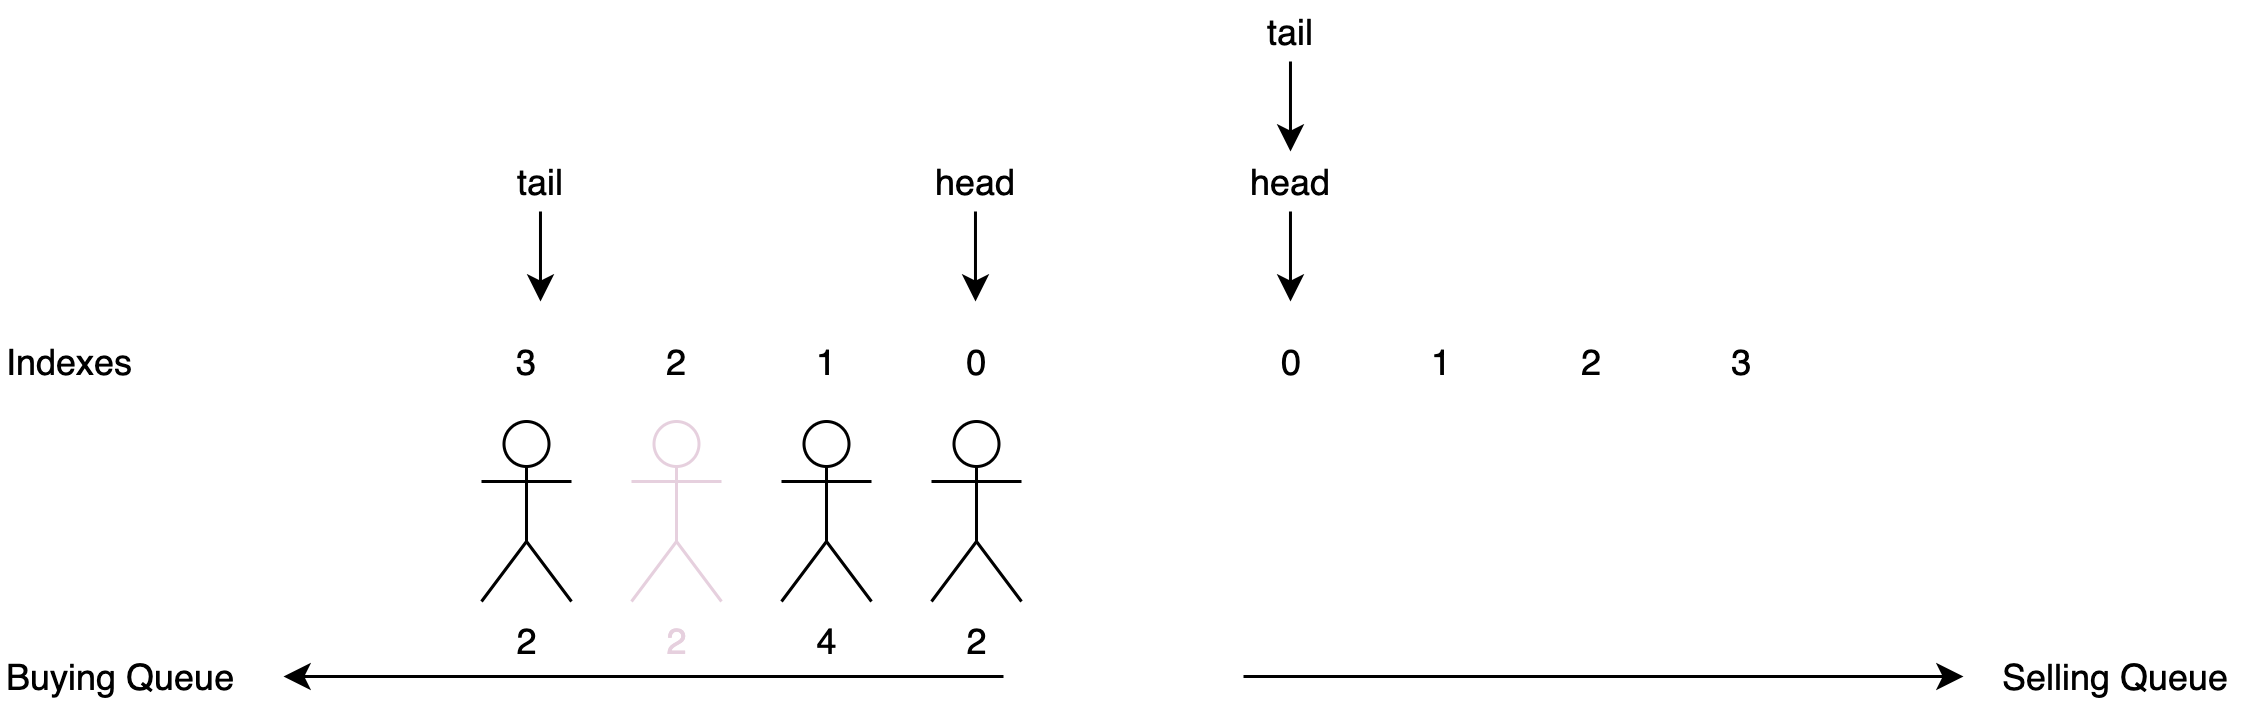
\includegraphics[width=16cm]{figures/aftermarket-queue.png}
    \caption{Aftermarket with buying and selling queue}
    \label{fig:aftermarket-queue}
\end{figure}

An important note to make is that an order might run into an \textit{out-of-gas exception}, if many consecutive buyers or sellers leave the queue because finding the head of the queue takes multiple loop iterations. In such a scenario, the users has to iterate over all the users that left the queue before finding a buyer/seller. 

This problem can be solved by adding function to the SC that reads how many people must be skipped before finding an actual buyer/seller. This must be a read-only function and does not cost any network fees. The result of read operation can be used to set an adequate network fee for the buy/sell order. 

\subsection{Dynamic Pricing}
To allow dynamic pricing below the original price, an architecture was designed to accomplish multiple buying and selling queues with fixed prices. The creator of an event can configure the aftermarket with an arbitrary number of queues. However, it is a trade-off between granular pricing and the possibility of allowing a black market to emerge. When configuring too many queues, it is possible to facilitate a trade between a buyer and seller from the black market. This can be achieved by selecting a pair of buying and selling queue which both are empty similar to the scenario explained in an open order book in Section \ref{section:aftermarket}. When configuring too little queues, the end user is restricted in setting the desired reselling price. 

The fixed prices are defined by using a percentage of the original prices and the granularity can be configured by the event owner. 

The following scenarios describe possible states of the aftermarket. Figure \ref{fig:aftermarket-high-demand} shows how multiple people queued up in the buying queues meaning that the demand for this type of ticket is high. A ticket owner can immediately sell his ticket to any person at the head of each queue. Of course to maximize profit, one should always choose the queue that offers the highest price.

\begin{figure}[H]
    \centering
    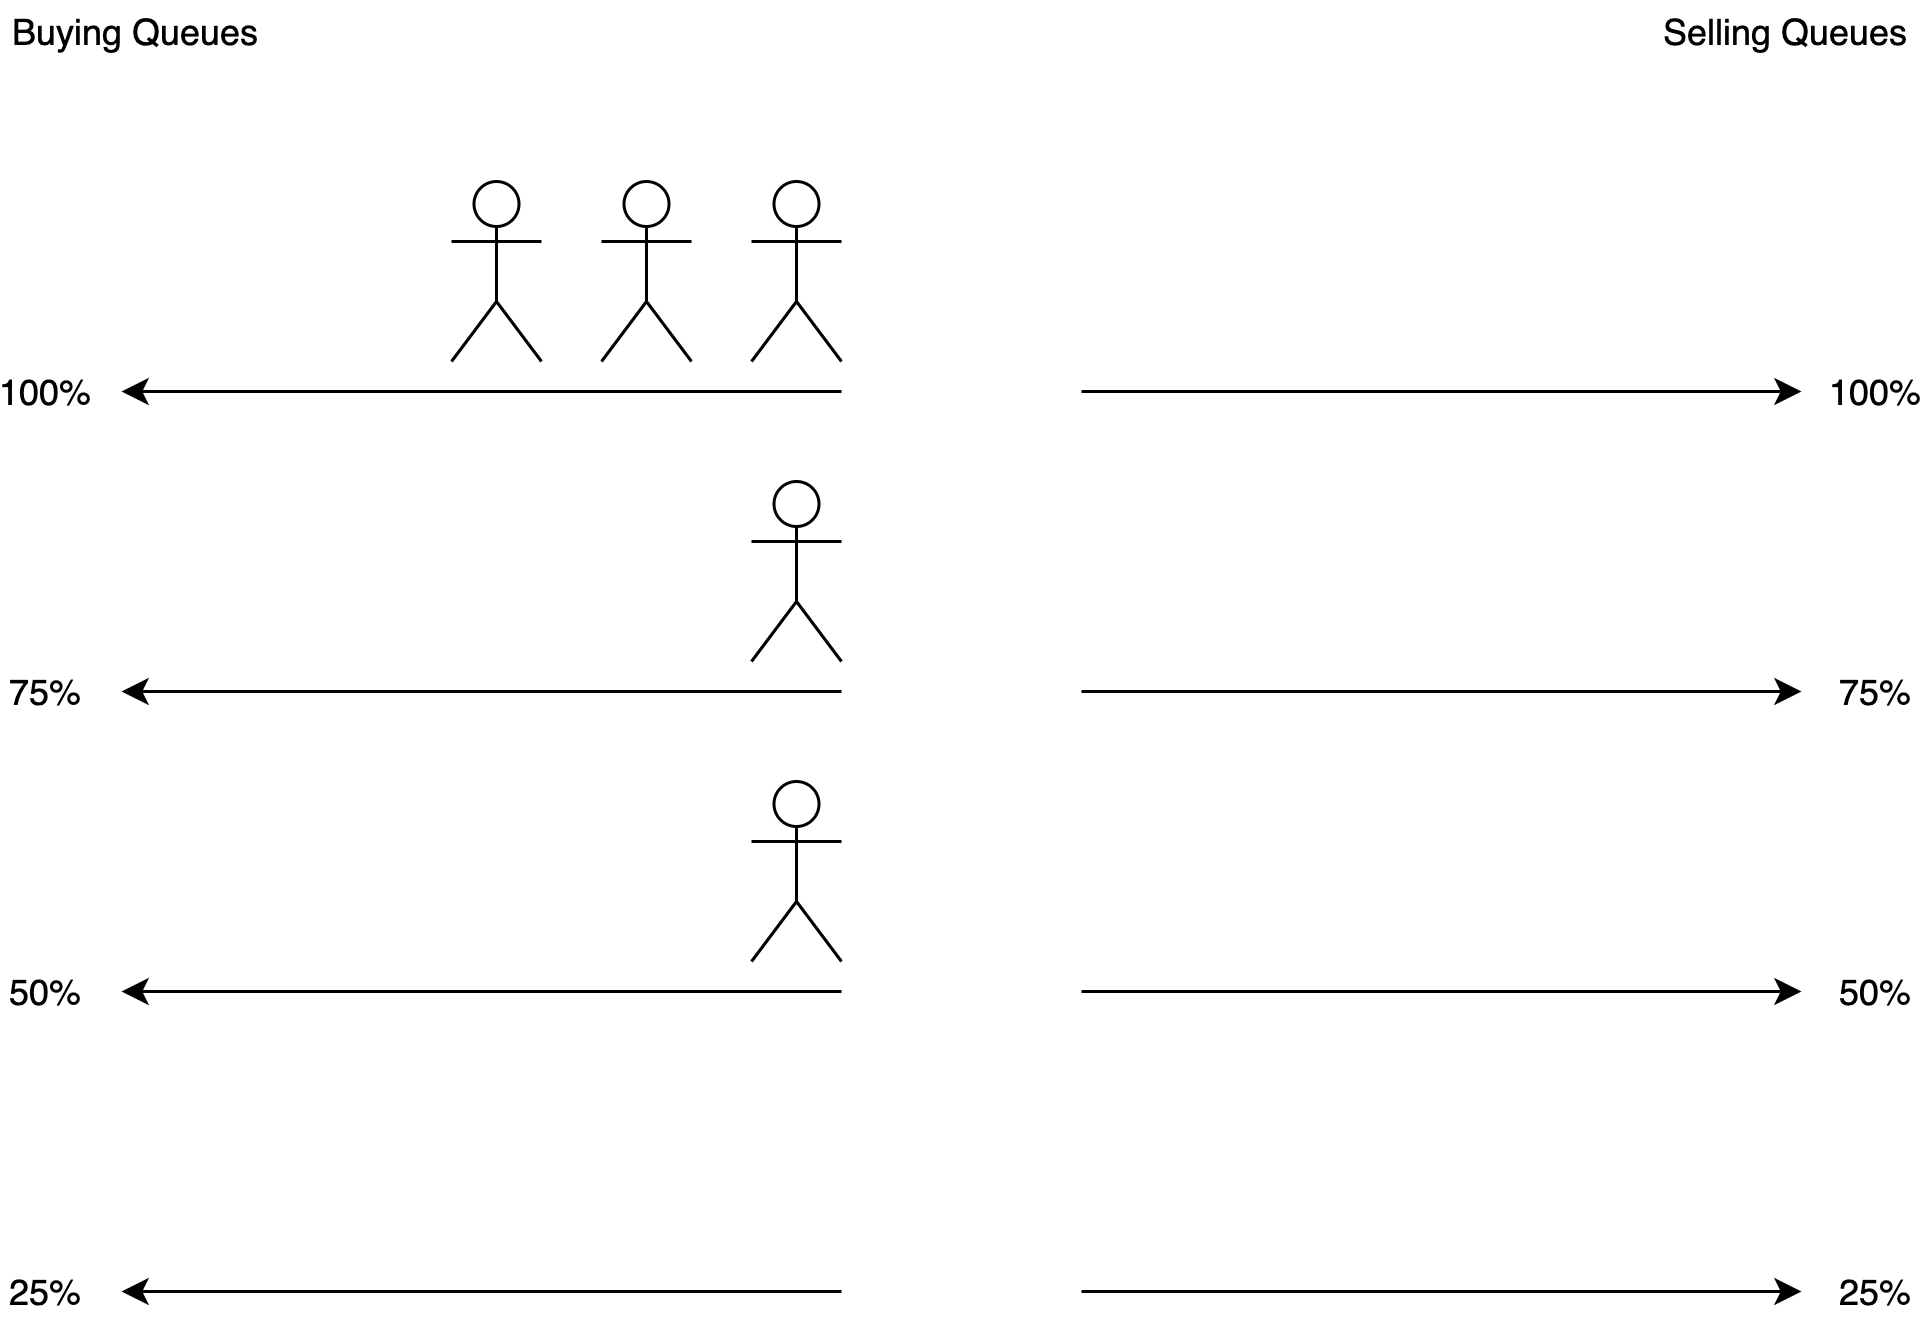
\includegraphics[width=12cm]{figures/aftermarket-high-demand.png}
    \caption{Aftermarket with high demand}
    \label{fig:aftermarket-high-demand}
\end{figure}

Contrarily, the same state can occur in the selling queues. Meaning that the supply is higher than the demand. A buyer can instantly fill a sell order.

It is also possible that the aftermarket levels at a lower price than the original ticket price. This is shown in Figure \ref{fig:aftermarket-mixed} where multiple people are willing to sell the ticket for 75\% of the original price. On the other side, multiple people are willing to buy a ticket for only 50\% of the original ticket price. In this state, any seller could immediately settle a trade at 50\% of the original price and any buyer could immediately fill an offer at 75\%. 

\begin{figure}[H]
    \centering
    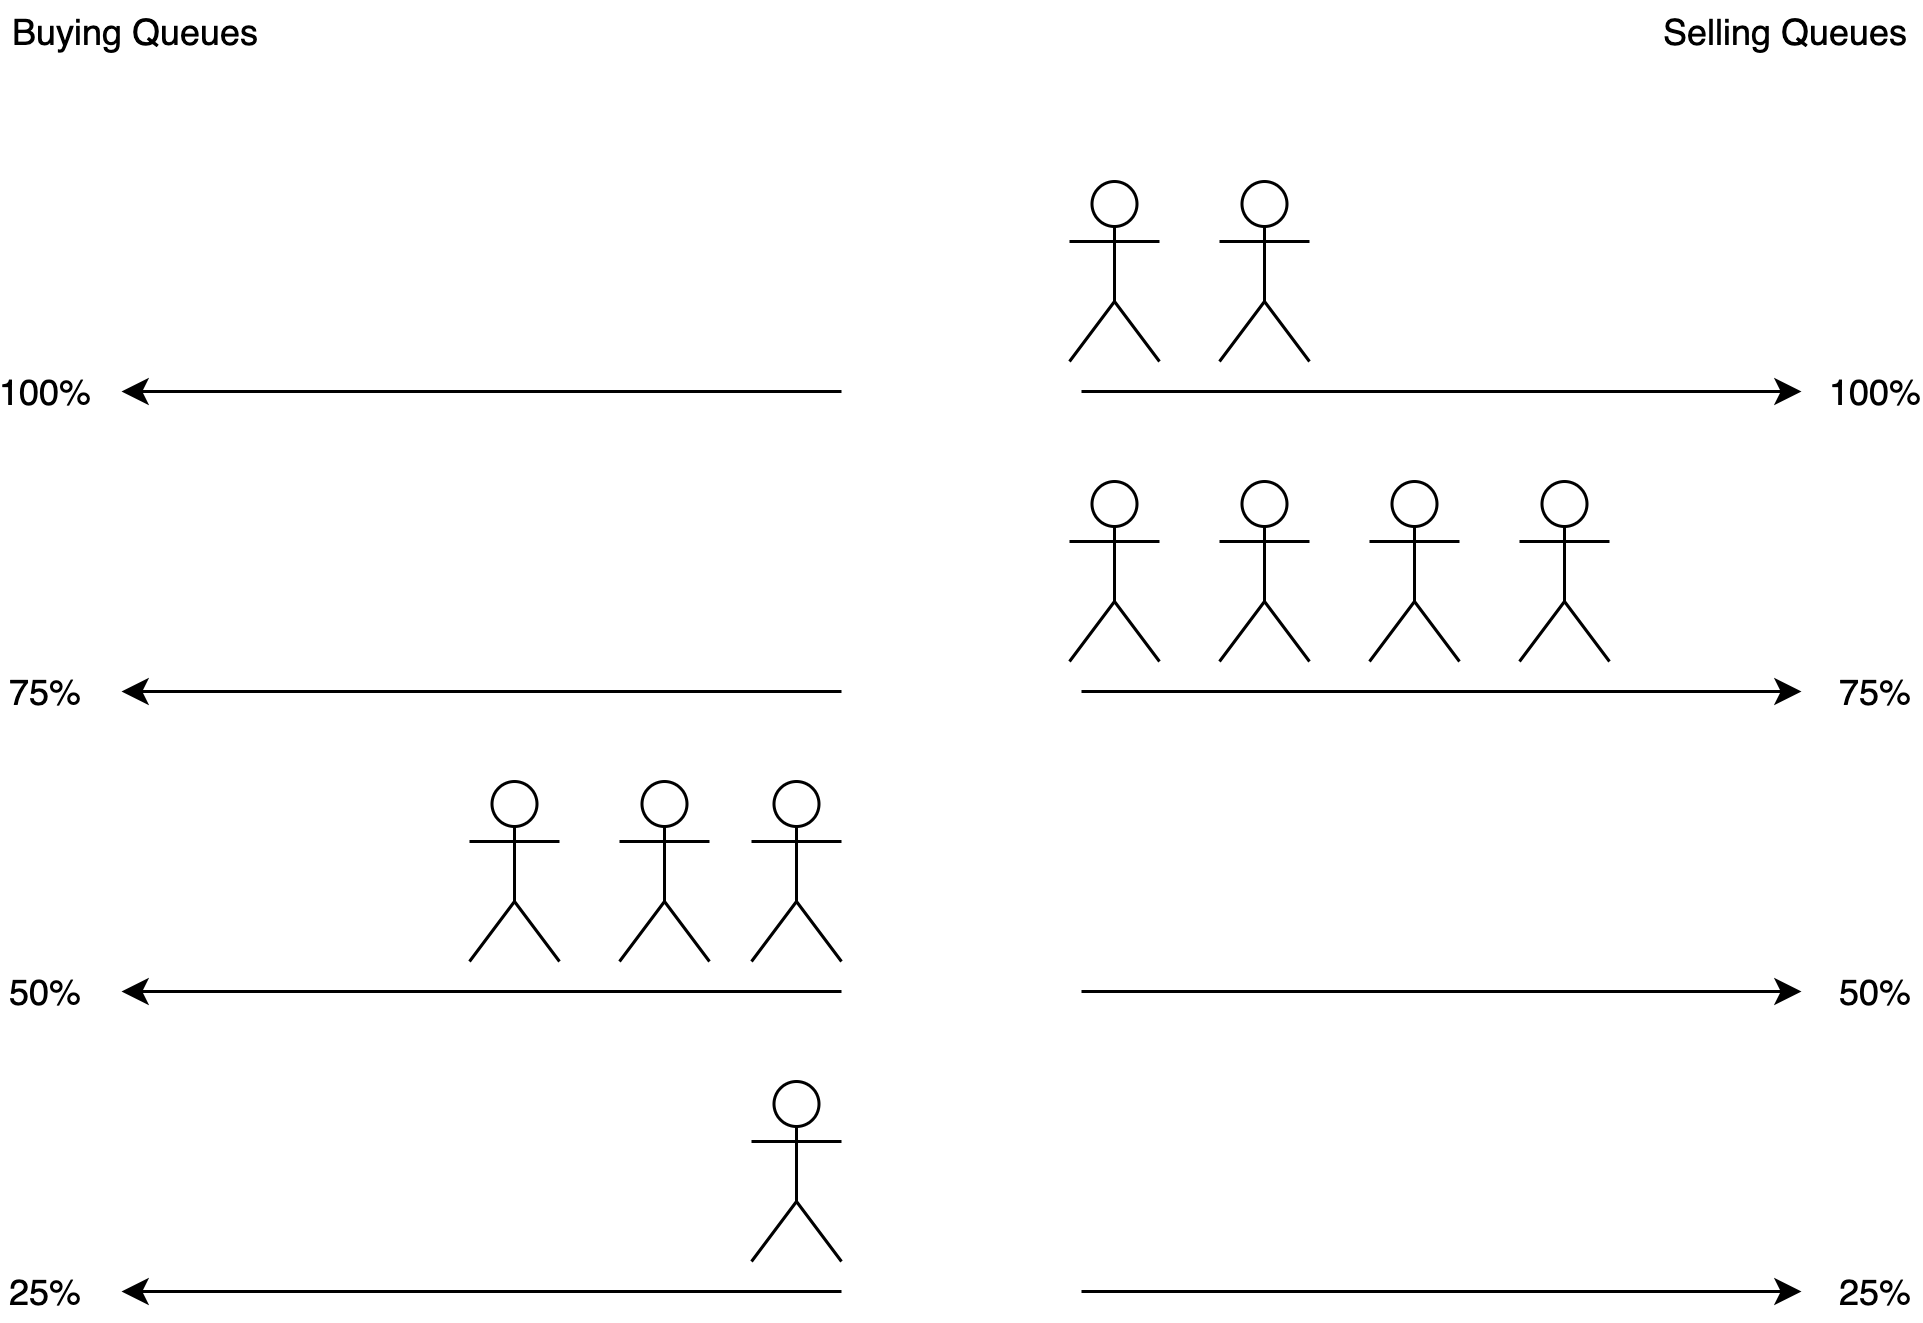
\includegraphics[width=12cm]{figures/aftermarket-mixed.png}
    \caption{Aftermarket with lower prices than original ticket price}
    \label{fig:aftermarket-mixed}
\end{figure}

Another scenario that is possible can occur when people join the wrong queue. This can occur when a sell and a buy order is processed in the same block or due to wrongful interaction with the SC. Such a state of the aftermarket is shown in Figure \ref{fig:aftermarket-arbitrage}. There is a person willing to sell a ticket for less than the highest offer on the buyer side. This opens the possibility of arbitrage trading. A third person can buy the ticket at 50\% and immediately resell the ticket again for 75\%. 

\begin{figure}[H]
    \centering
    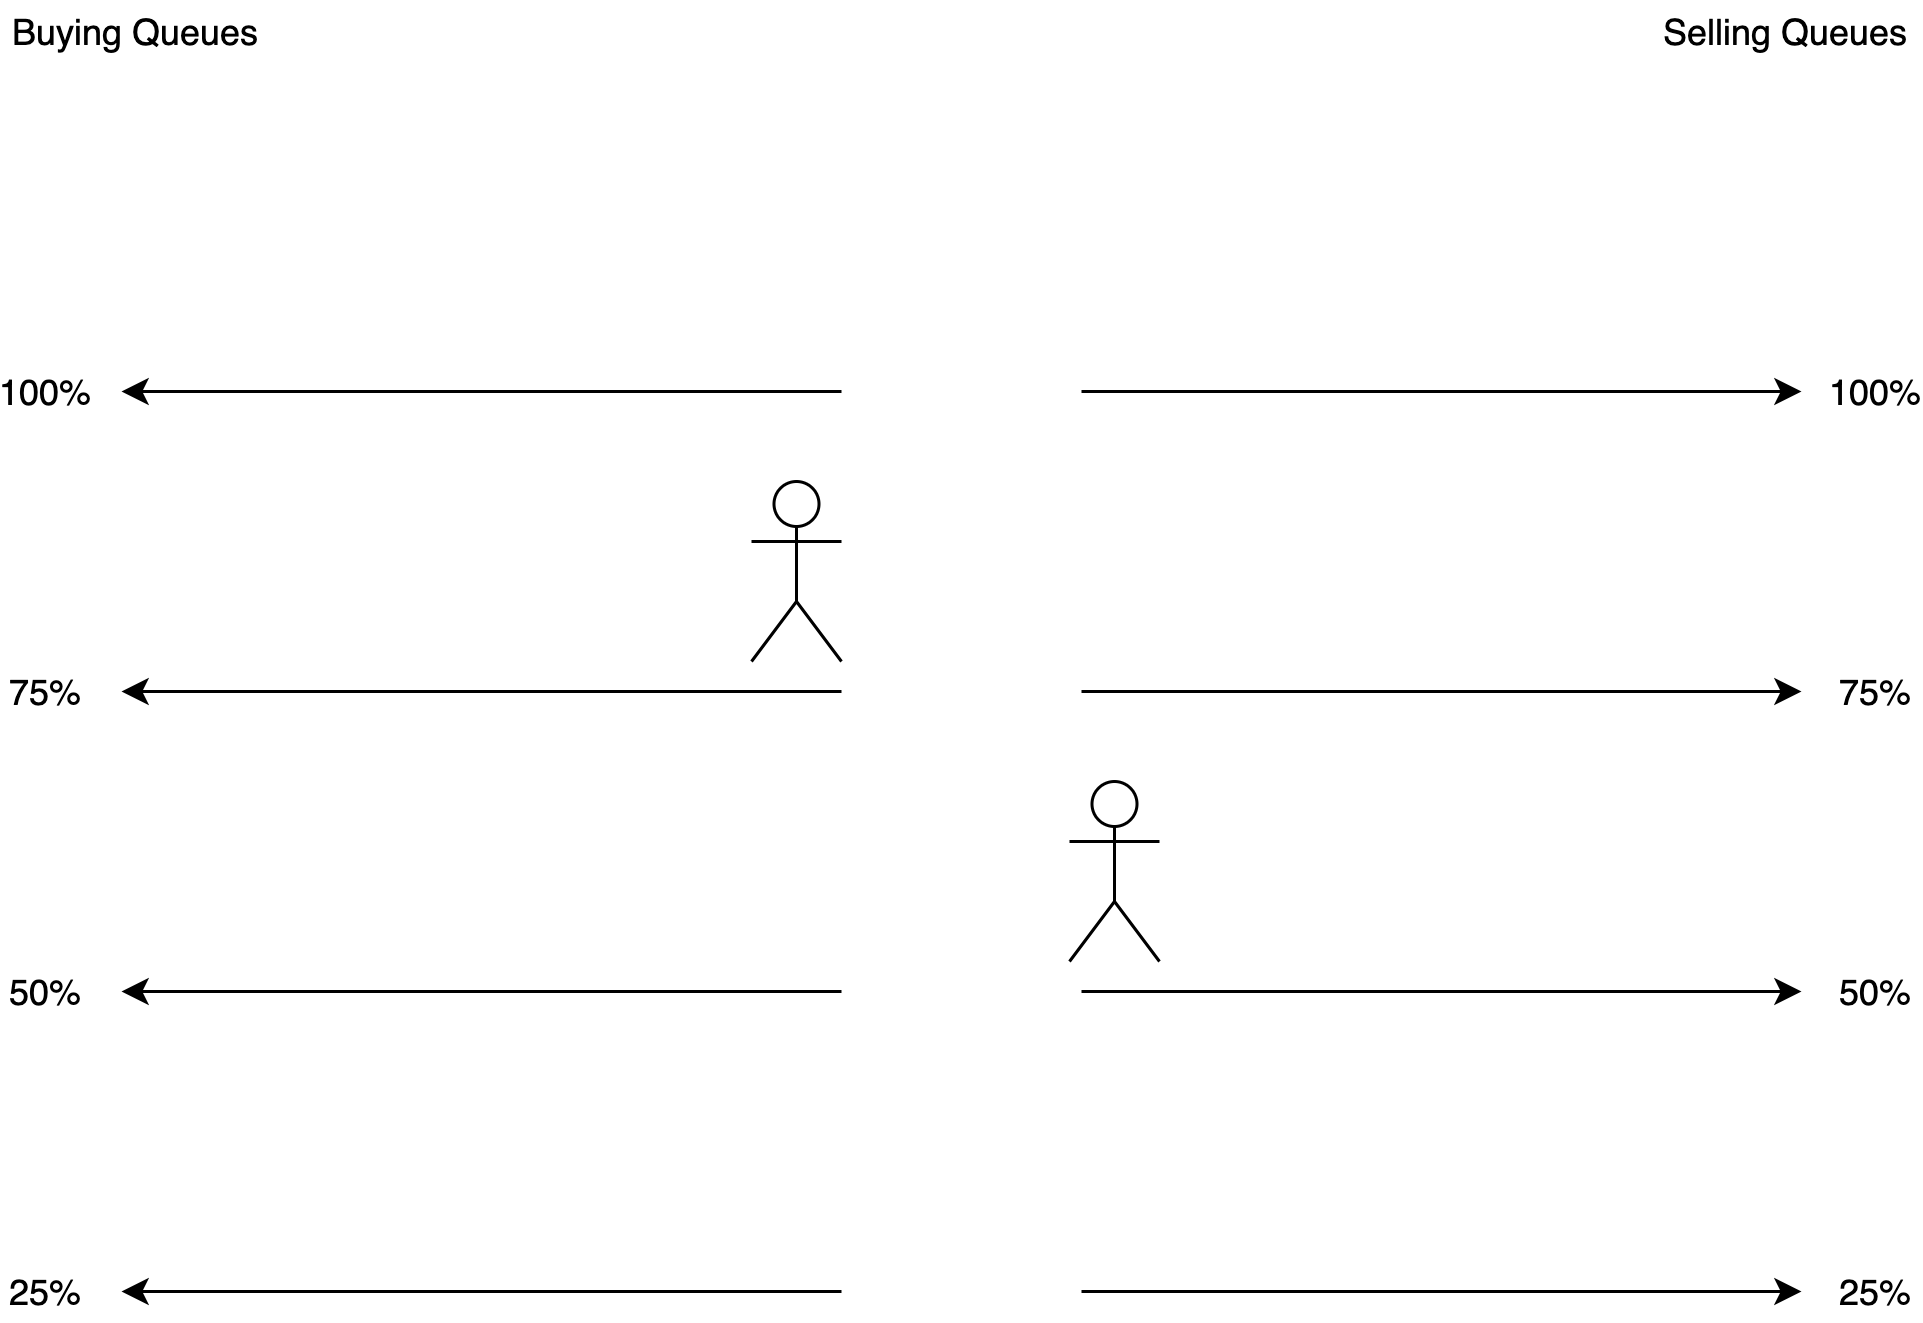
\includegraphics[width=12cm]{figures/aftermarket-arbitrage.png}
    \caption{Aftermarket with arbitrage opportunities}
    \label{fig:aftermarket-arbitrage}
\end{figure}

There are two solutions to solve that problem. Joining the wrong queue due to human error can be eliminated by warning the user in the frontend application that joining the selected queue results in a loss of opportunity cost. 

Solving the issue in the SC comes at the price of efficiency. Additional parameter can be introduced to keep track how many people are in each queue. Before each trade, the SC evaluates if the described state occurs. However, depending on the granularity of the queues, it might not be feasible to loop over each queue as this results in higher network fees and might lead to an 
\textit{out-of-gas exception}.

In this project, a warning in the frontend is displayed when a user attempts to join a queue that is not optimal.

\subsection{Presale}\label{section:des:presale}
Whenever an event takes place and the demand for the tickets is high, the potential guests will try to buy the tickets when the sale period starts. This leads to a high traffic on the ticket sellers website. It is then also not clear, which person can finish the buying process and is often determined by the internet speed of their internet service provider.

To prevent this problem and to have fair and clear odds for every guest, a lottery system for the initial ticket distribution is put in place. Every guest, that wants to attend the event, can place a buy order during the presale. This order will cost as much as the ticket. At the end of the presale period, the tickets will be distributed using a random number, in the case a guest has not won a ticket, he then will be able to reclaim the spent money. If there are more tickets than interested buyers in the presale, each of them receives a ticket. 

The design pattern of the \textit{future blockhash} is used to generate a random number. During the creation of a presale ticket type, a future blocknumber is defined. This block acts as the closing date for the presale as well as the source of randomness. This design patter is a good fit due to its simplicity. There is a chance of manipulation by the miner that adds the block with the defined number by not publishing a block if randomness is not in his favour. However, in order to do so, the miner must resign on the block reward. If this is an actual threat to a ticketing platform, the prices have to be larger than the ticket price. 

\subsection{ERC Standard}
All three ERC standard explained in Section \ref{subsubsection:token-interfaces} require a function which allows the owner to transfer the token/ticket to another address of his choice. Without explicitly deactivating this function, people are able to sell the ticket on a different platform for higher prices and consequently, allowing a secondary market to emerge. The goal of this project is that there exists only one marketplace/exchange for each event operating transparently on the BC. Also, tickets must not transferred in the same way as these ERC standards do.

It is be possible to deactivate the transfer function or whitelist a specific exchange address such that tickets could only be sold through this exchange. However, this breaks the design principle of these ERC standards. These standards are developed to create a common interface such that a token can be used across multiple exchanges and the usability is the same among different tokens. Also, tickets must only be resold in one contract to minimize the risk of emerging a black market (see Section \ref{section:aftermarket}). Merging the event logic with the aftermarket logic in one contract has a positive side-effect that no extra transaction is needed to approve the aftermarket (DEX). 

Furthermore, the logic for approving and storing other exchanges increases the complexity of the event SC and becomes more expensive to create and deploy a new event.These are the reasons for not implementing any of the ERC interfaces for the event contract and instead creating a new contract from scratch. 


\subsection{Economics}\label{design:economy}

The economic model works differently in a decentralized system. The entire business logic is stored in public SC that anybody can fork and redeploy. With the proposed design an event host does not need any hardware or software infrastructure to create an event and issue tickets. However, other stakeholders play a crucial role in the ticketing process as shown in the diagram \ref{fig:dlt-based-landscape}.

The host either relies on trustworthy ID approvers or does his own KYC procedure. To incentivize ID approvers to become trustworthy and to compensate them for their service, a fraction of each ticket price is directly paid to the selected ID approver. Since this is an open design ID approvers compete with others to become popular among the event hosts.

Furthermore, the same principle applies for the GUI builders. Anybody can interact with the SC. This can either be done directly with the command line interface (CLI) or using a GUI. A GUI provider is also compensated for his service if the ticket is bought through his application. This creates a fair competition among different GUI builder.

Affiliates are companies or influential people that promote an event. Affiliates are also included in the buying process and are being compensated with a direct payment for each ticket that is bought due to their service. 


\begin{figure}[H]
    \centering
    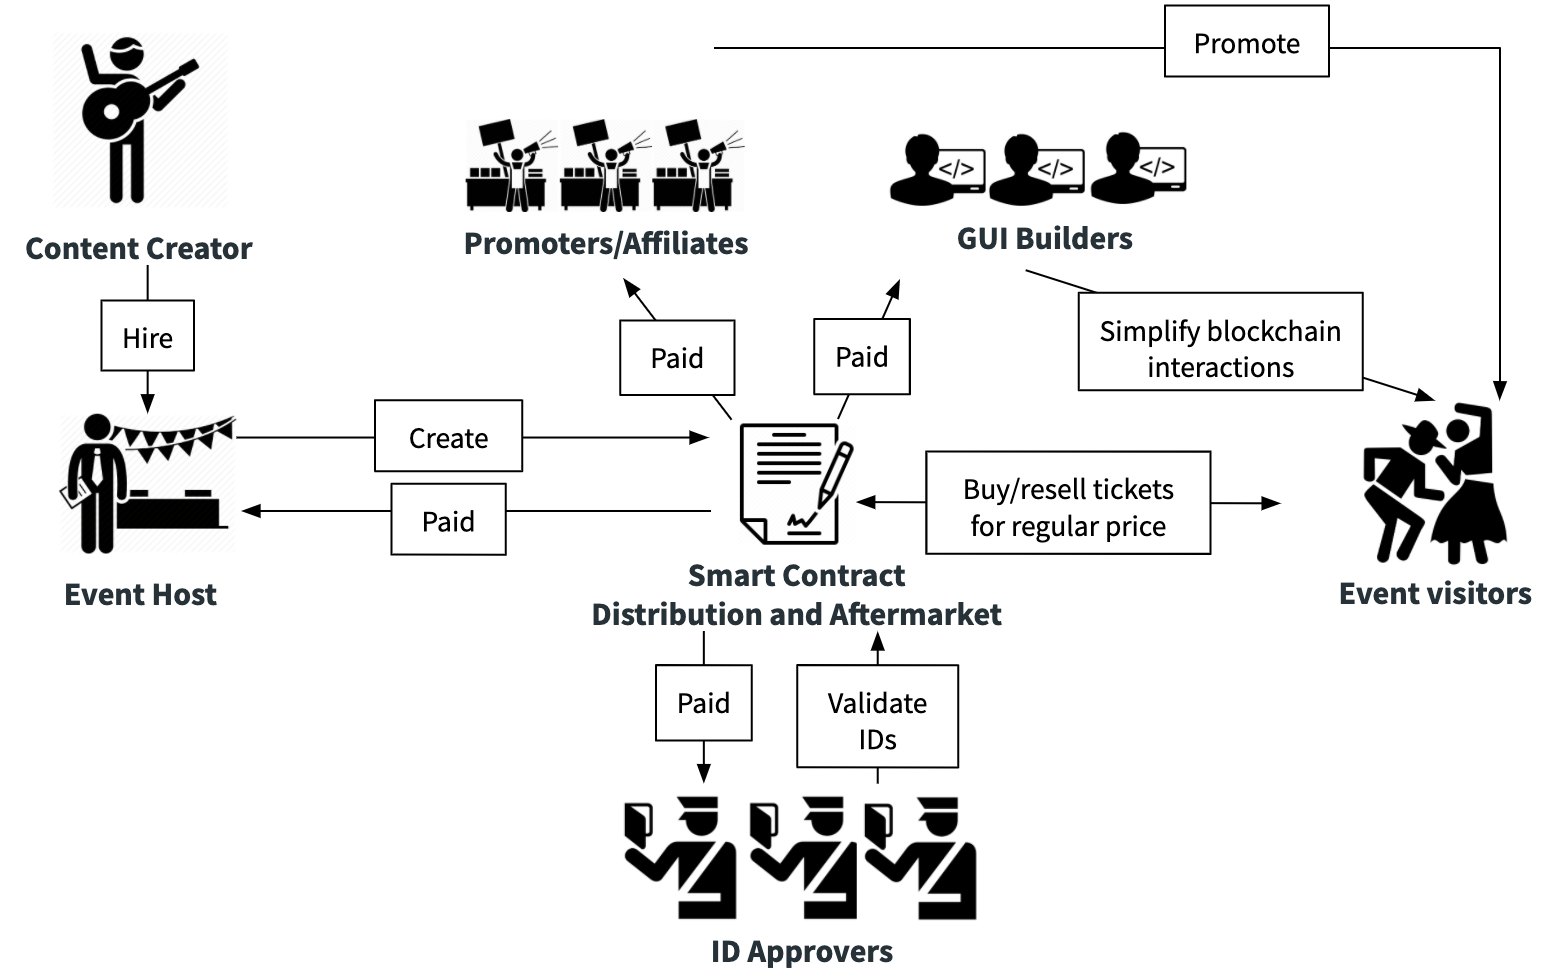
\includegraphics[width=16cm]{figures/dlt-based-landscape.png}
    \caption{DLT-based architecture}
    \label{fig:dlt-based-landscape}
\end{figure}

